%************************************************
\chapter{Case Study}\label{ch:evaluation}
%************************************************
Part of the evaluation of the developed tool is to verify the functionality with an existing company. In order to do so, a company closely related to the University of Groningen has been found. This company is named `Sustainable Buildings' and sells products to monitor the users electricity and gas consumption in real-time. This leads to an increase in building-users awareness by providing real-time feedback through public dashboards \cite{sb}.\\

\noindent
In order to provide this monitoring, they have allocated a physical server consisting of 40 cores and 128 GB of RAM. Additionally, they have 900 GB of storage data. This host machine is divided into 6 virtual machines. A brief overview of their architecture is described in \autoref{sec:sb-architecture}. The decision has been made to deploy the developed tool at their system, because it is a relatively large system with many load. Additionally, the tool might be useful for them, as they are now missing insights into their performance. The process of deploying this system has been described in \autoref{sec:sb-process}. At the end, an evaluation has been performed. This evaluation consists of an interview and is described in \autoref{sec:sb-evaluation}.

\section{Architecture} \label{sec:sb-architecture}
The six virtual machines work together as one system. Each virtual machine is responsible for running a number of services. These services can be found in \autoref{fig:sb-architecture}. In order to simplify the deployment, the decided to assign a name to every VM. The names are also presented in the architecture diagram. A small overview of the number of CPU, RAM and memory per VM can be found in \autoref{tab:vms}.\\

\noindent
As described in \autoref{sec:collect_utilization}, the architecture is a fully connected peer-to-peer system, as well as a hierarchical structure for the data replication. For the latter, the structure can be found in \autoref{fig:sb-tree}.


\begin{figure}
    \centering
    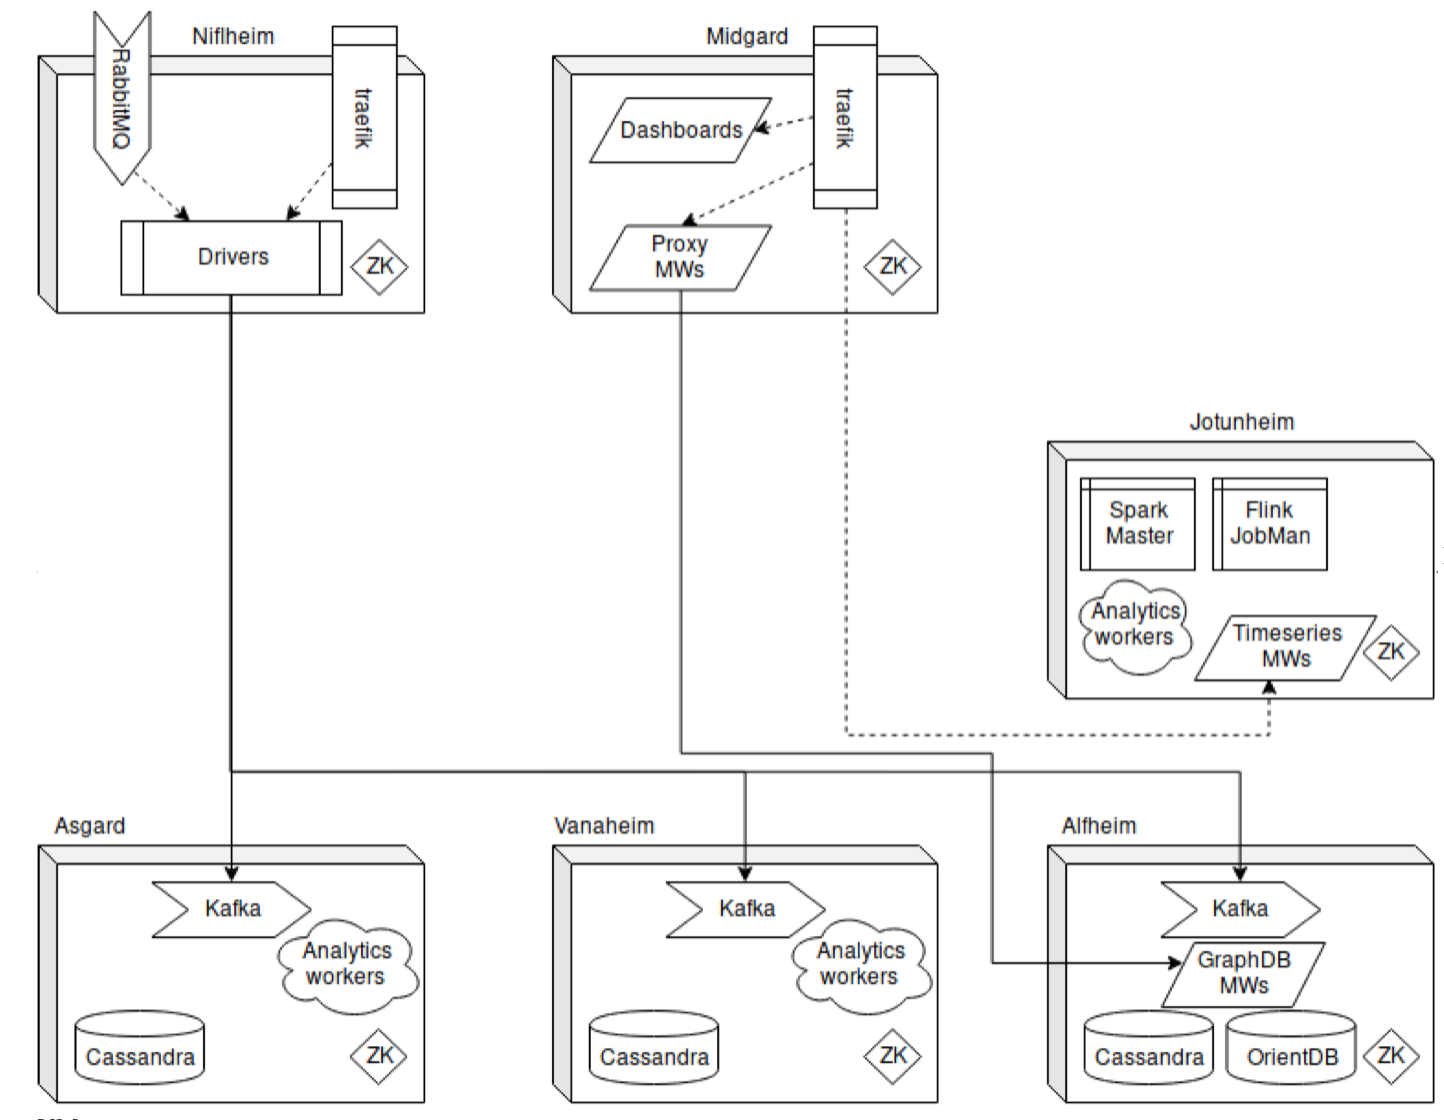
\includegraphics[width=\textwidth]{gfx/sb-architecture.png}
    \caption{Sustainable Buildings architecture}
    \label{fig:sb-architecture}
\end{figure}

\begin{table}
    \centering
    \begin{tabular}{l|rrr}
        Virtual Machine & Cores & RAM & Memory \\ \hline
        Midgard & 4 & 8 GB & 20 GB \\
        Niflheim & 4 & 8 GB & 20 GB \\
        Jotunheim & 8 & 16 GB & 100 GB \\
        Asgard & 8 & 16 GB & 100 GB \\
        Vanaheim & 8 & 16 GB & 100 GB \\
        Alfheim & 8 & 16 GB & 100 GB \\
    \end{tabular}
    \caption{Overview of their architecture}
    \label{tab:vms}
\end{table}

\begin{figure}
    \centering
    \begin{forest}
        for tree={
            grow=south,
            rectangle, draw, minimum size=3ex, inner sep=1pt,s sep=7mm
        }
        [Alfheim 
            [Vanaheim 
                [Asgard]
            ]
            [Midgard
                [Jotunheim]
                [Niffelheim]
            ]
        ]
    \end{forest}
    \caption{Hierarchical overview of the Case study}
    \label{fig:sb-tree}
\end{figure}

\section{Deployment process} \label{sec:sb-process}
This section describes the process of deploying the implemented system on their architecture. This deployment has been made possible within three meetings. They are shortly described in the sub-sections below.

\subsection{First meeting}
Each meeting consisted of three hours. After the first meeting, there were several issues. Initially, the developed system was implemented in such a way that the nodes were communicating over their public IP address. However, it turned out that not every node was publicly accessible. Therefore, the program was updated, such that they communicate over their internal IP. Another issue was due to the amount of load going in and out their system. Therefore, the part of the program that monitors the internet traffic with respect to the containers raised its CPU to above 100\% as can be seen in \autoref{fig:100}.
The decision was therefore made to not deploy the program any more, and first solve the issues that showed up.

\begin{figure}
    \centering
    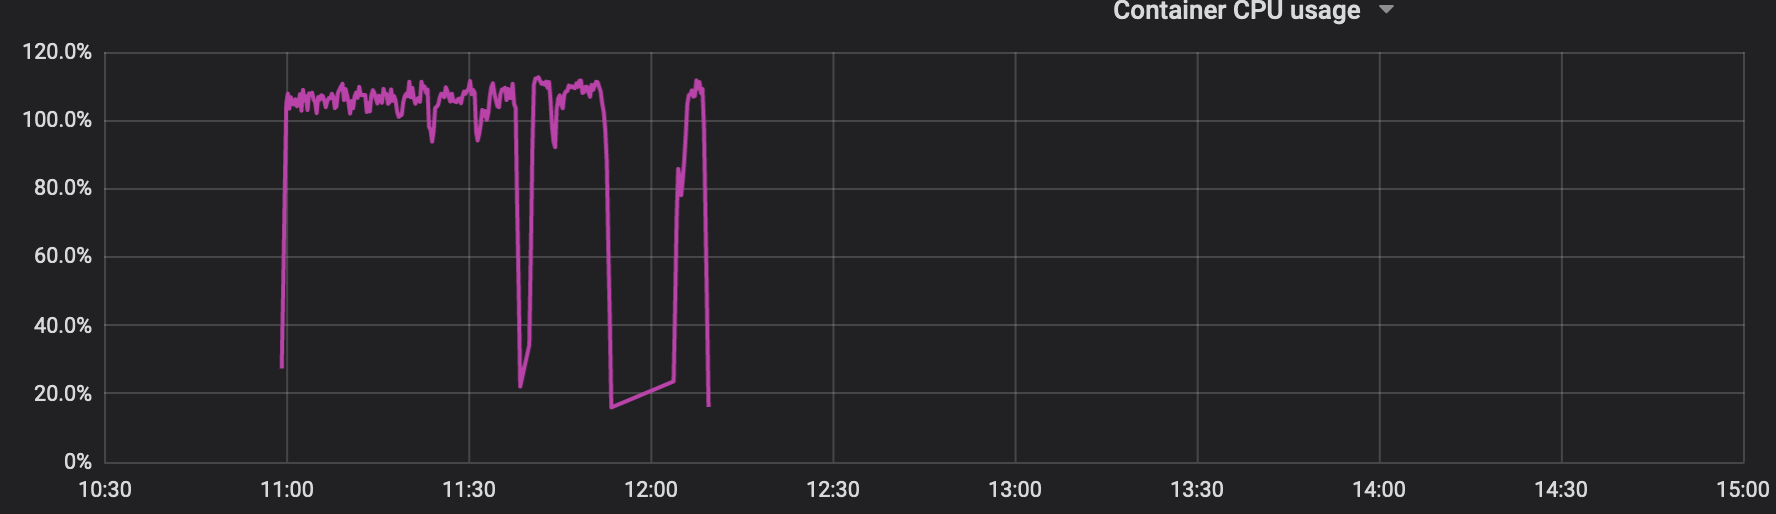
\includegraphics[width=\textwidth]{gfx/load-100.png}
    \caption{CPU data of the deployed system during the first meeting}
    \label{fig:100}
\end{figure}

\subsection{Second meeting}
In order to solve the issue described in the previous sub-section, a sub sampling of the internet monitoring was applied. Therefore, instead of capturing all packets, the packets where captured for $x$ seconds, while sleeping $y$ seconds. The packet size collected during each sampling was therefore multiplied with $1+y/x$. However, for every packet that is coming from a peer within the system, the program tries to assign this packet directly to a remote Docker container. Therefore, there was still a significant amount of communication overhead, which can be seen in \autoref{fig:60}. Eventually, the program kept consuming more CPU resources, which lead to the conclusion that the program was not efficient enough. Therefore, the program was not deployed.

\begin{figure}
    \centering
    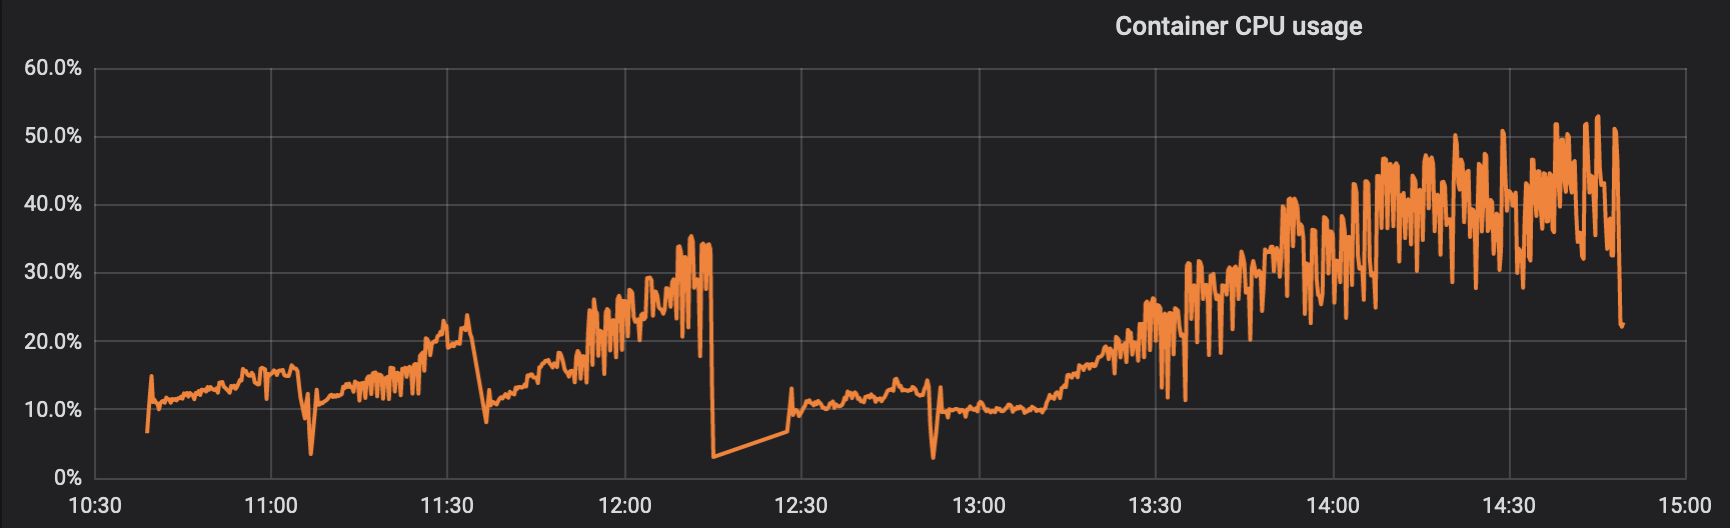
\includegraphics[width=\textwidth]{gfx/load-60.png}
    \caption{CPU data of the deployed system during the second meeting}
    \label{fig:60}
\end{figure}

\subsection{Third meeting}
In order to solve the issue from the second meeting, the decision was made to implement a caching functionality. This means that the program resolves the internet traffic packets afterwards instead of real-time. The decision was made to implement a caching time limit of one minute, such that the obtained results are near real-time. The system therefore only communicates with its peer once per minute. It turned out that this optimization was efficient enough, as the program showed an average of 10\% CPU usage during the entire deployment of the system. This can be seen in \autoref{fig:deployment}. In this figure, a random moment (from 9 AM to 11 AM) was taken to show the 

\begin{figure}
    \subfloat[Asgard]{%
        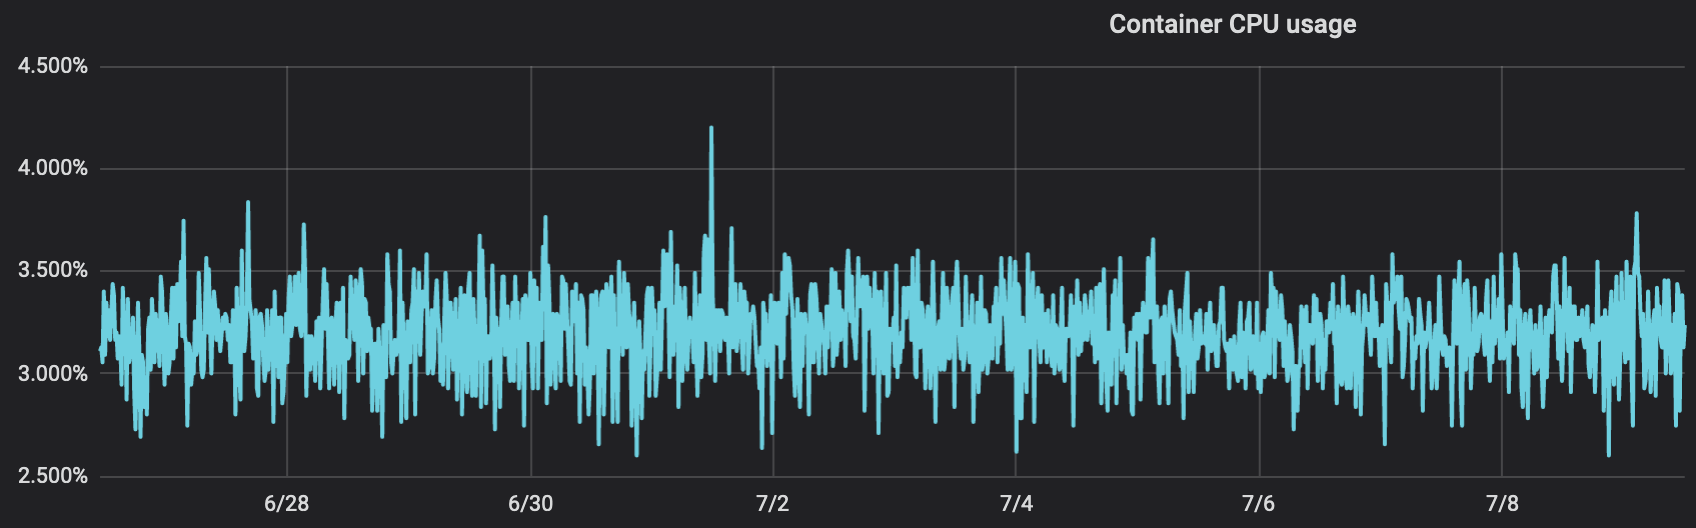
\includegraphics[width=0.45\textwidth]{gfx/asgard.png}
        \label{fig:deployment:asgard}
    }\qquad
    \subfloat[Midgard]{
        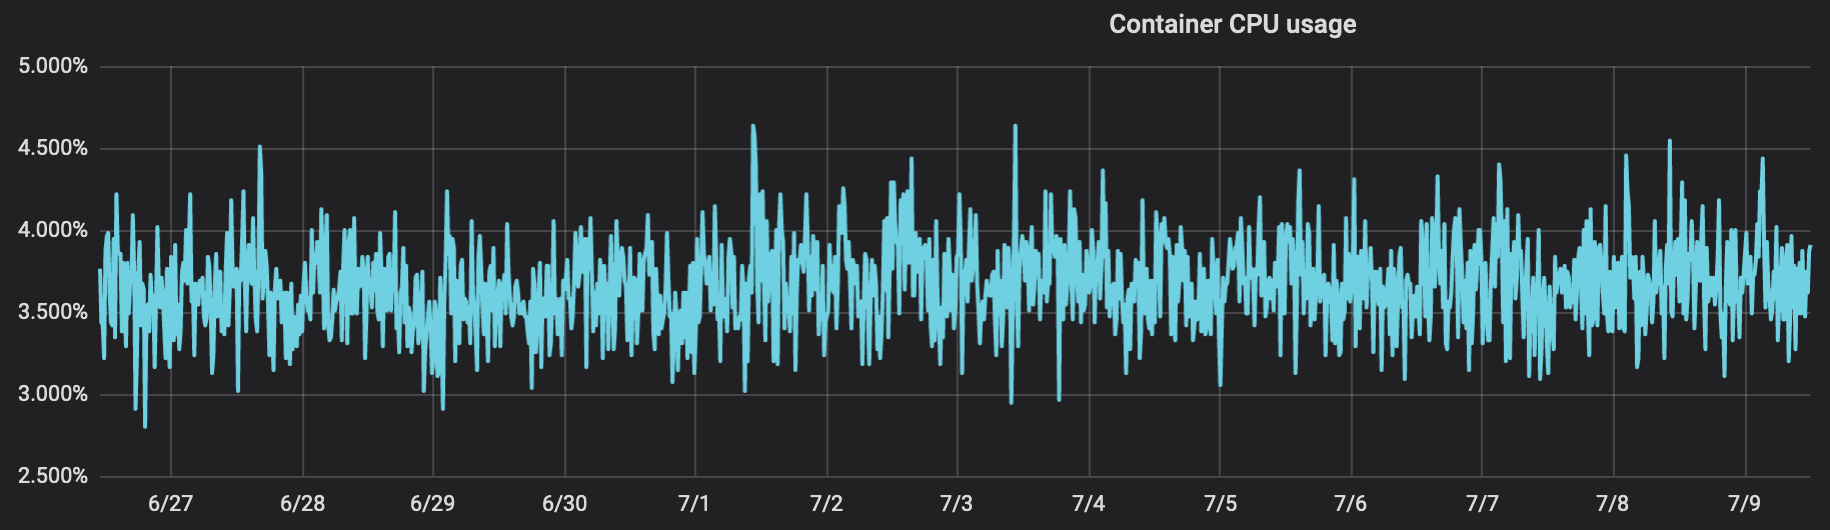
\includegraphics[width=0.45\textwidth]{gfx/midgard.png}%
        \label{fig:deployment:midgard}
    }

    \subfloat[Vanaheim]{%
        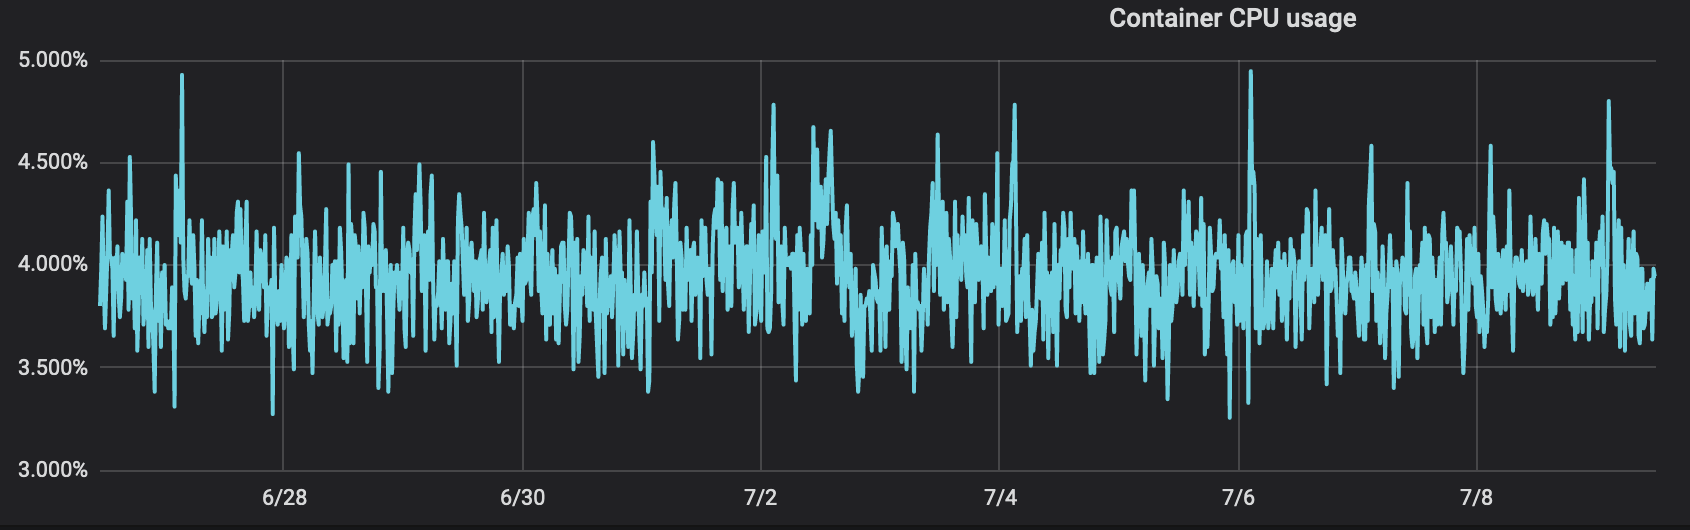
\includegraphics[width=0.45\textwidth]{gfx/vanaheim.png}
        \label{fig:deployment:vanaheim}
    }\qquad
    \subfloat[Alfheim]{
        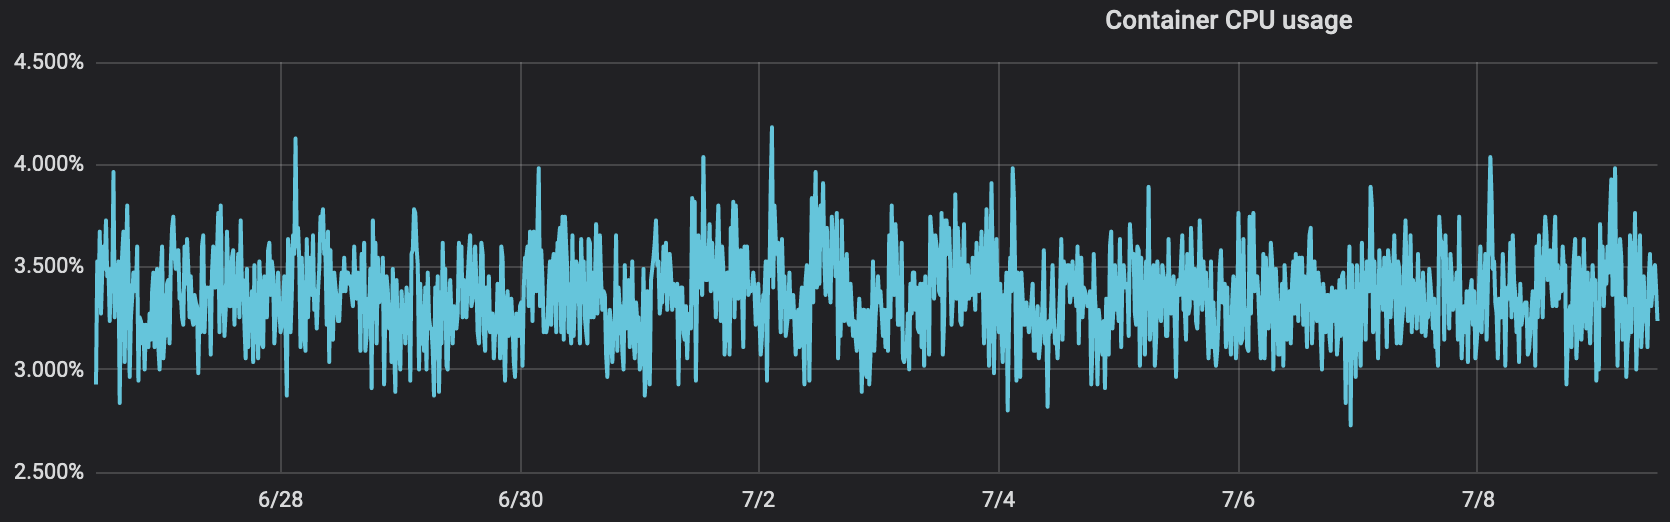
\includegraphics[width=0.45\textwidth]{gfx/alfheim.png}%
        \label{fig:deployment:alfheim}
    }
    
    \subfloat[Jotunheim]{%
        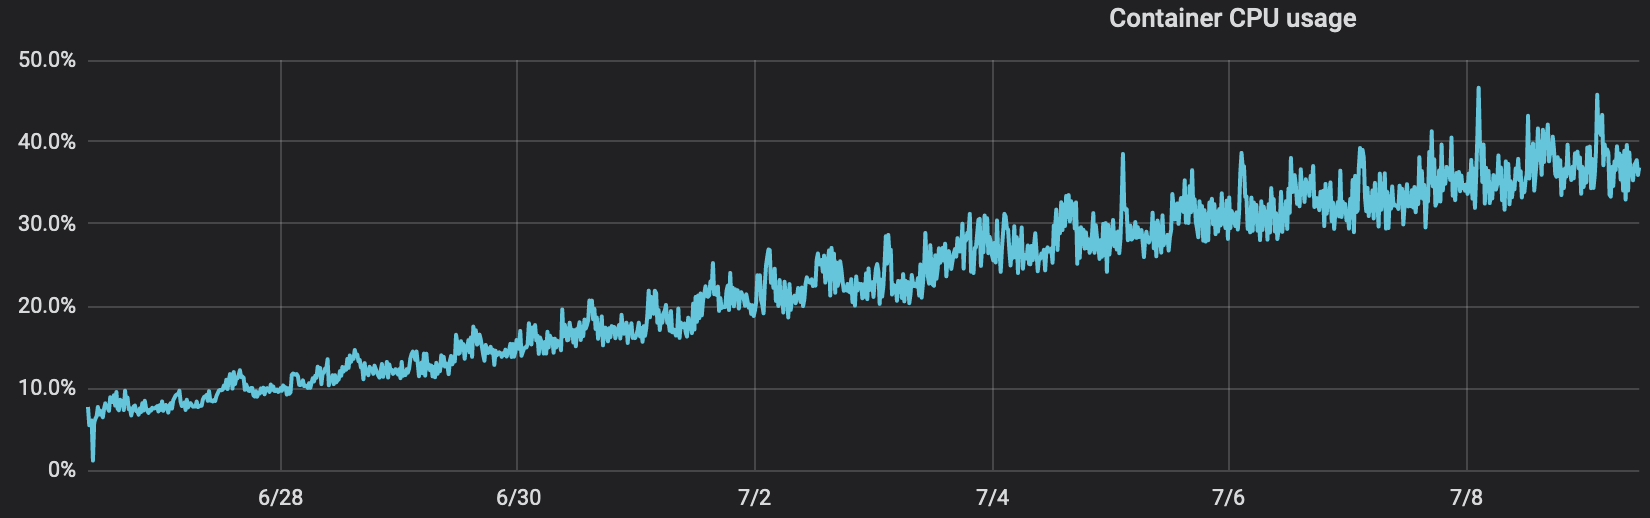
\includegraphics[width=0.45\textwidth]{gfx/jotunheim.png}
        \label{fig:deployment:jotunheim}
    }\qquad
    \subfloat[Niflheim]{
        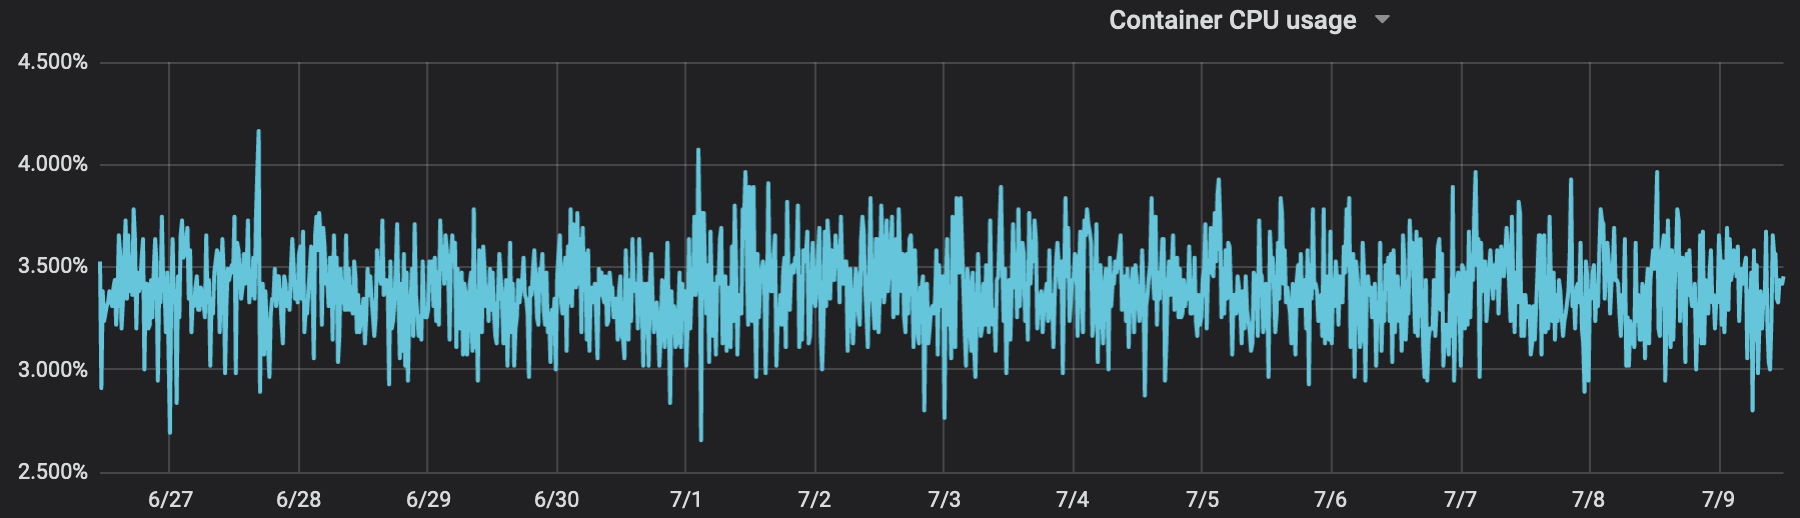
\includegraphics[width=0.45\textwidth]{gfx/niflheim.png}%
        \label{fig:deployment:niflheim}
    }
    \caption{CPU utilization of the deployed system at 6 different VMs.}
    \label{fig:deployment}
\end{figure}


\section{Evaluation} \label{sec:sb-evaluation}
In order to evaluate the deployment of the system, the decision has been made to perform an interview with one of the employees of the company. The entire interview can be found in \autoref{ch:interview}.